% Options for packages loaded elsewhere
\PassOptionsToPackage{unicode}{hyperref}
\PassOptionsToPackage{hyphens}{url}
\PassOptionsToPackage{dvipsnames,svgnames,x11names}{xcolor}
%
\documentclass[
  a4paper,
]{article}

\usepackage{amsmath,amssymb}
\usepackage{iftex}
\ifPDFTeX
  \usepackage[T1]{fontenc}
  \usepackage[utf8]{inputenc}
  \usepackage{textcomp} % provide euro and other symbols
\else % if luatex or xetex
  \usepackage{unicode-math}
  \defaultfontfeatures{Scale=MatchLowercase}
  \defaultfontfeatures[\rmfamily]{Ligatures=TeX,Scale=1}
\fi
\usepackage{lmodern}
\ifPDFTeX\else  
    % xetex/luatex font selection
\fi
% Use upquote if available, for straight quotes in verbatim environments
\IfFileExists{upquote.sty}{\usepackage{upquote}}{}
\IfFileExists{microtype.sty}{% use microtype if available
  \usepackage[]{microtype}
  \UseMicrotypeSet[protrusion]{basicmath} % disable protrusion for tt fonts
}{}
\makeatletter
\@ifundefined{KOMAClassName}{% if non-KOMA class
  \IfFileExists{parskip.sty}{%
    \usepackage{parskip}
  }{% else
    \setlength{\parindent}{0pt}
    \setlength{\parskip}{6pt plus 2pt minus 1pt}}
}{% if KOMA class
  \KOMAoptions{parskip=half}}
\makeatother
\usepackage{xcolor}
\usepackage[top=2.54cm,right=2.54cm,bottom=2.54cm,left=2.54cm]{geometry}
\setlength{\emergencystretch}{3em} % prevent overfull lines
\setcounter{secnumdepth}{-\maxdimen} % remove section numbering
% Make \paragraph and \subparagraph free-standing
\ifx\paragraph\undefined\else
  \let\oldparagraph\paragraph
  \renewcommand{\paragraph}[1]{\oldparagraph{#1}\mbox{}}
\fi
\ifx\subparagraph\undefined\else
  \let\oldsubparagraph\subparagraph
  \renewcommand{\subparagraph}[1]{\oldsubparagraph{#1}\mbox{}}
\fi


\providecommand{\tightlist}{%
  \setlength{\itemsep}{0pt}\setlength{\parskip}{0pt}}\usepackage{longtable,booktabs,array}
\usepackage{calc} % for calculating minipage widths
% Correct order of tables after \paragraph or \subparagraph
\usepackage{etoolbox}
\makeatletter
\patchcmd\longtable{\par}{\if@noskipsec\mbox{}\fi\par}{}{}
\makeatother
% Allow footnotes in longtable head/foot
\IfFileExists{footnotehyper.sty}{\usepackage{footnotehyper}}{\usepackage{footnote}}
\makesavenoteenv{longtable}
\usepackage{graphicx}
\makeatletter
\def\maxwidth{\ifdim\Gin@nat@width>\linewidth\linewidth\else\Gin@nat@width\fi}
\def\maxheight{\ifdim\Gin@nat@height>\textheight\textheight\else\Gin@nat@height\fi}
\makeatother
% Scale images if necessary, so that they will not overflow the page
% margins by default, and it is still possible to overwrite the defaults
% using explicit options in \includegraphics[width, height, ...]{}
\setkeys{Gin}{width=\maxwidth,height=\maxheight,keepaspectratio}
% Set default figure placement to htbp
\makeatletter
\def\fps@figure{htbp}
\makeatother

\makeatletter
\makeatother
\makeatletter
\makeatother
\makeatletter
\@ifpackageloaded{caption}{}{\usepackage{caption}}
\AtBeginDocument{%
\ifdefined\contentsname
  \renewcommand*\contentsname{Tabla de contenidos}
\else
  \newcommand\contentsname{Tabla de contenidos}
\fi
\ifdefined\listfigurename
  \renewcommand*\listfigurename{Listado de Figuras}
\else
  \newcommand\listfigurename{Listado de Figuras}
\fi
\ifdefined\listtablename
  \renewcommand*\listtablename{Listado de Tablas}
\else
  \newcommand\listtablename{Listado de Tablas}
\fi
\ifdefined\figurename
  \renewcommand*\figurename{Figura}
\else
  \newcommand\figurename{Figura}
\fi
\ifdefined\tablename
  \renewcommand*\tablename{Tabla}
\else
  \newcommand\tablename{Tabla}
\fi
}
\@ifpackageloaded{float}{}{\usepackage{float}}
\floatstyle{ruled}
\@ifundefined{c@chapter}{\newfloat{codelisting}{h}{lop}}{\newfloat{codelisting}{h}{lop}[chapter]}
\floatname{codelisting}{Listado}
\newcommand*\listoflistings{\listof{codelisting}{Listado de Listados}}
\makeatother
\makeatletter
\@ifpackageloaded{caption}{}{\usepackage{caption}}
\@ifpackageloaded{subcaption}{}{\usepackage{subcaption}}
\makeatother
\makeatletter
\@ifpackageloaded{tcolorbox}{}{\usepackage[skins,breakable]{tcolorbox}}
\makeatother
\makeatletter
\@ifundefined{shadecolor}{\definecolor{shadecolor}{rgb}{.97, .97, .97}}
\makeatother
\makeatletter
\makeatother
\makeatletter
\makeatother
\ifLuaTeX
\usepackage[bidi=basic]{babel}
\else
\usepackage[bidi=default]{babel}
\fi
\babelprovide[main,import]{spanish}
% get rid of language-specific shorthands (see #6817):
\let\LanguageShortHands\languageshorthands
\def\languageshorthands#1{}
\ifLuaTeX
  \usepackage{selnolig}  % disable illegal ligatures
\fi
\usepackage[]{biblatex}
\addbibresource{../../../../references.bib}
\IfFileExists{bookmark.sty}{\usepackage{bookmark}}{\usepackage{hyperref}}
\IfFileExists{xurl.sty}{\usepackage{xurl}}{} % add URL line breaks if available
\urlstyle{same} % disable monospaced font for URLs
\hypersetup{
  pdftitle={Pautas para la presentación del informe de investigación en economía enfoque, estructura y elementos clave},
  pdfauthor={Edison Achalma},
  pdflang={es},
  colorlinks=true,
  linkcolor={blue},
  filecolor={Maroon},
  citecolor={Blue},
  urlcolor={Blue},
  pdfcreator={LaTeX via pandoc}}

\title{Pautas para la presentación del informe de investigación en
economía enfoque, estructura y elementos clave}
\usepackage{etoolbox}
\makeatletter
\providecommand{\subtitle}[1]{% add subtitle to \maketitle
  \apptocmd{\@title}{\par {\large #1 \par}}{}{}
}
\makeatother
\subtitle{Guía práctica para estudiantes de economía en la elaboración
de informes de investigación}
\author{Edison Achalma}
\date{2023-06-03}

\begin{document}
\maketitle
\ifdefined\Shaded\renewenvironment{Shaded}{\begin{tcolorbox}[sharp corners, interior hidden, boxrule=0pt, borderline west={3pt}{0pt}{shadecolor}, frame hidden, breakable, enhanced]}{\end{tcolorbox}}\fi

\hypertarget{introducciuxf3n}{%
\section{Introducción}\label{introducciuxf3n}}

Al iniciar el semestre académico, es fundamental que los alumnos definan
de manera precisa el objetivo de su trabajo de investigación y evalúen
su relevancia, factibilidad y valor agregado. Se recomienda tomar estas
decisiones después de revisar la literatura básica y explorar la
disponibilidad de información estadística sobre el tema de
investigación.

La investigación económica abarca una amplia diversidad y depende de la
formación, capacidad y motivación del investigador. Algunos ejemplos de
tipos de investigación incluyen:

\begin{enumerate}
\def\labelenumi{\arabic{enumi}.}
\item
  Comprobación de hipótesis: En esta modalidad, el alumno presenta una
  hipótesis acerca de un fenómeno económico y busca comprobarla en su
  trabajo de investigación. Por ejemplo: ``En la economía peruana, el
  mecanismo de transmisión de la política monetaria no es el canal de la
  tasa de interés, sino el canal del crédito''.
\item
  Estudio de relaciones: Aquí, el alumno plantea el problema y se enfoca
  en determinar las relaciones entre variables económicas. Por ejemplo:
  ¿Cuál es la relación entre las exportaciones y el crecimiento
  económico en el Perú? ¿Cuáles son los determinantes del tipo de cambio
  real en el Perú?
\item
  Formulación de modelos: En esta modalidad, el alumno formula o
  reformula modelos para la economía peruana con el objetivo de explicar
  el comportamiento de variables económicas. Por ejemplo: Formulación de
  un modelo macroeconómico que explique la determinación de salarios,
  precios y empleo en el corto plazo.
\end{enumerate}

A continuación, se presenta una estructura sugerida para la presentación
del informe de investigación.

\textbf{I. Planteamiento del problema}

\begin{figure}

\caption{\label{fig-1}Imagen 1}

{\centering 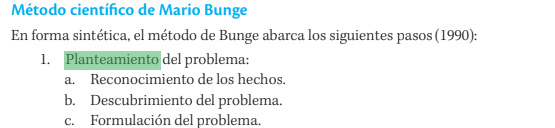
\includegraphics{20230603152205.png}

}

\end{figure}

En esta sección, el estudiante, después de revisar la bibliografía
relevante y los datos estadísticos relacionados con el problema
económico a estudiar, llevará a cabo:

Análisis cuantitativo y/o cualitativo del comportamiento de la variable
endógena (diagnóstico) - en este caso, el Producto Bruto Interno (PBI)
nacional, Impuesto Selectivo al Consumo (ISC), Impuesto General a las
Ventas (IGV), Impuesto a la Renta (IR) y otros impuestos.

Identificación de las causas del comportamiento de la variable endógena,
basado en la relación existente entre la variable endógena y la variable
exógena (explicación) - se puede emplear el método de Granger-MCO para
esto.

Exposición de propuestas de política económica basadas en la explicación
anterior (recomendación).

Formulación de preguntas que motiven respuestas en función del
diagnóstico, explicación y recomendación.

\textbf{II. Objetivos}

En esta sección, el estudiante debe presentar de manera clara sus
propósitos, tanto objetivos generales como específicos. Estos objetivos
deben formularse después de responder las siguientes preguntas:

\begin{enumerate}
\def\labelenumi{\arabic{enumi}.}
\tightlist
\item
  ¿Qué se desea lograr con la investigación?
\item
  ¿Qué conocimientos se busca adquirir?
\item
  ¿Qué se pretende demostrar?
\end{enumerate}

Es importante destacar que las respuestas a estas preguntas deben
contribuir a responder las interrogantes planteadas al final del
planteamiento del problema.

\textbf{III. Importancia y justificación}

En esta sección, el alumno expone las razones por las cuales plantea la
investigación. Estas motivaciones pueden tener un carácter teórico,
metodológico o práctico. Además, se pueden abordar las siguientes
interrogantes: \footnote{Para esta sección, resulta útil revisar Mendez
  (1995), páginas 92-97.}

\begin{itemize}
\tightlist
\item
  ¿Cuáles son los beneficios obtenidos al realizar esta investigación?
\item
  ¿Por qué resulta necesaria esta investigación?
\item
  ¿A quiénes beneficiará?
\item
  ¿Quiénes serán los potenciales usuarios?
\end{itemize}

\textbf{IV. Antecedentes}

En esta parte, el alumno debe revisar y presentar los trabajos de
investigación empírica relacionados con el tema. En general, es esencial
presentar una síntesis de dichos estudios, haciendo énfasis en los
objetivos, la metodología utilizada, las conclusiones y las
recomendaciones.

\textbf{V. Consideraciones teóricas}

En esta sección, el alumno debe presentar la literatura teórica
relevante al problema seleccionado.

\textbf{VI. Hipótesis}

En esta parte, el alumno, basándose en los elementos teóricos expuestos
anteriormente, plantea una proposición de causa (variable exógena) y
efecto (variable endógena). Cabe recordar que una hipótesis en modelos
estáticos se traduce en palabras a partir de los resultados de los
ejercicios de estática comparativa.

\textbf{VII. Metodología y datos}

En esta sección, el alumno:

\begin{enumerate}
\def\labelenumi{\arabic{enumi}.}
\tightlist
\item
  Identifica el método a utilizar.
\item
  Identifica el tipo de investigación a realizar.
\item
  Presenta las variables económicas identificadas empíricamente.
\item
  Señala las fuentes de información y/o la forma de recopilación de los
  datos.
\item
  Describe el proceso de procesamiento de la información.
\end{enumerate}

\textbf{VIII. Esquema}

En esta parte, el alumno presentará el esquema de la estructura del
trabajo de investigación por capítulos. En cada capítulo, es necesario
identificar los objetivos específicos correspondientes.

\textbf{IX. Desarrollo del esquema de investigación}

En esta sección, los alumnos, basándose en gráficos, tablas, técnicas
estadísticas y econométricas, obtienen conclusiones y plantean
recomendaciones en cada capítulo del esquema planteado.

\textbf{X. Bibliografía}

Aquí el alumno presenta la lista de obras consultadas que han servido
para fundamentar el planteamiento del problema, los antecedentes, el
marco teórico y las hipótesis.

\hypertarget{bibliografuxeda}{%
\section{Bibliografía}\label{bibliografuxeda}}

Méndez Álvarez, C. E. (1995). Metodología: guía para elaborar diseños de
investigación en ciencias económicas, contables y administrativas.
Buenos Aires, Argentina: McGraw-Hill.

Mendoza Bellido, W. E. (2007). Cómo investigan los economistas: Guía
para elaborar y desarrollar un proyecto de investigación. Fondo
Editorial, PUCP.


\printbibliography


\end{document}
